\section{Materials and Methods}
\label{sec:methods}

This section describes the corpus, the counting system, and the instrument we use to
measure it. The pipeline is deliberately conventional; the measurement is not, and it is
what makes the paper's central result visible.

\subsection{Dataset: Corpus, Annotation and Splits}
\label{sec:dataset}

The corpus is 32 nocturnal road-transect videos recorded with a vehicle-mounted FLIR
thermal camera across four sites in southern Illinois, eight videos per site. Frames are
$640\times512$ single-channel thermal at 60\,fps; the vehicle travels at 25--90\,km/h, so
the background translates continuously and the same animal is visible for a few seconds at
most. \Cref{fig:dataset} shows representative frames with their annotation, and
\cref{tab:dataset} summarizes the corpus. Showing the raw and annotated rows together is the
point: the annotation looks unambiguous once drawn, but the top row is what a detector
actually receives, and in its third and fourth panels the animals are a few dozen pixels of
slightly warmer texture against thermal clutter. The median animal is $29\times24$\,px,
approximately the smallest box in the third panel.

Thermal transects carry low and drifting global contrast, so every frame is normalized with contrast-limited adaptive histogram equalisation (CLAHE)~\cite{reza2004realization} before use, identically at training and inference and for
every model reported here. This single preprocessing choice is worth more than any architectural one we tested: test mAP50 falls from $0.519$ to $0.299$ without it, which
is why the figures in this paper show normalized rather than raw frames: they are the pixels
the detectors actually consume.

\begin{figure}[htbp]
\centering
\setlength{\tabcolsep}{1.5pt}
\renewcommand{\arraystretch}{0.6}
\begin{tabular}{cccc}
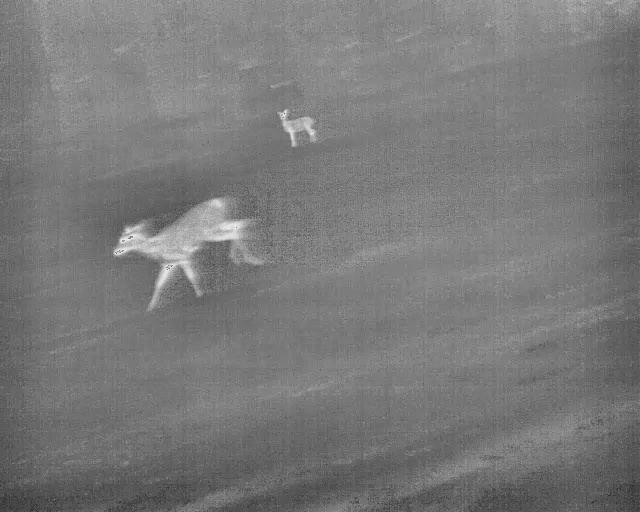
\includegraphics[width=0.228\textwidth]{figures/dataset/p1_raw.jpg} &
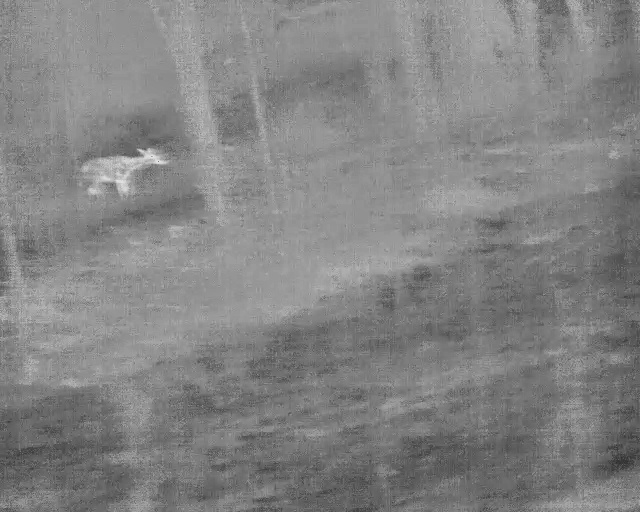
\includegraphics[width=0.228\textwidth]{figures/dataset/p2_raw.jpg} &
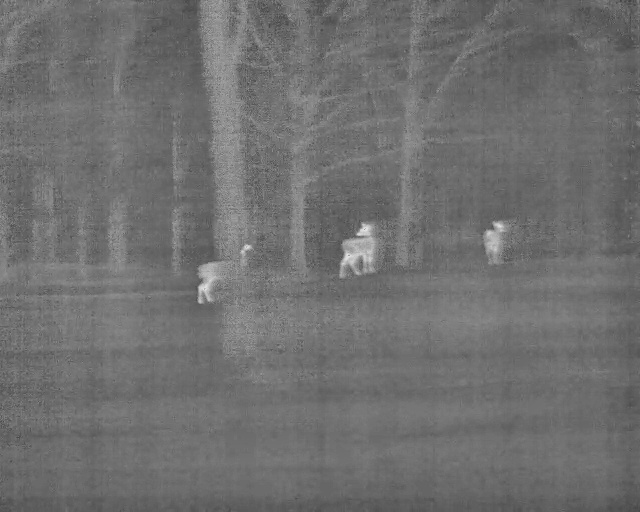
\includegraphics[width=0.228\textwidth]{figures/dataset/p3_raw.jpg} &
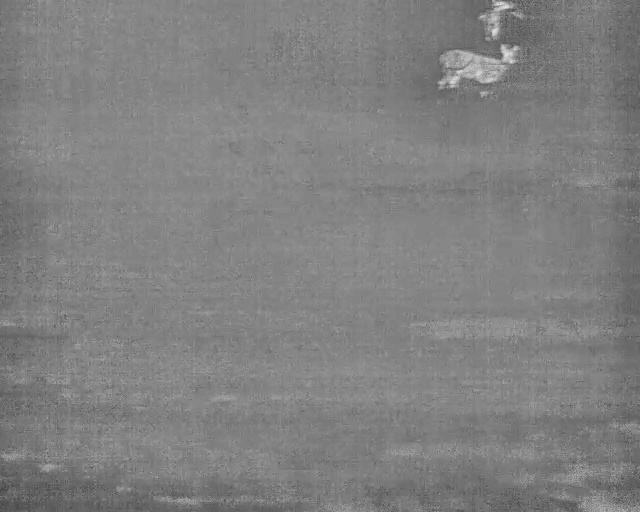
\includegraphics[width=0.228\textwidth]{figures/dataset/p4_raw.jpg} \\
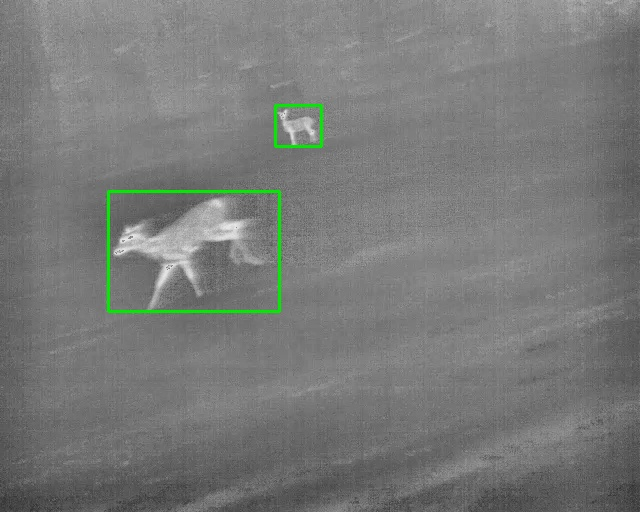
\includegraphics[width=0.228\textwidth]{figures/dataset/p1_gt.jpg} &
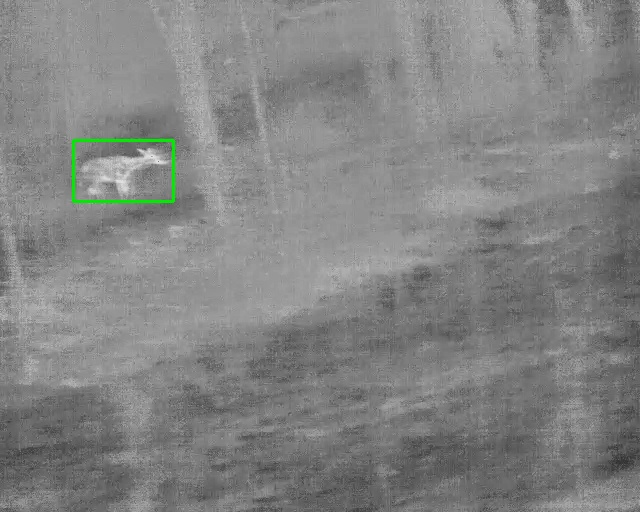
\includegraphics[width=0.228\textwidth]{figures/dataset/p2_gt.jpg} &
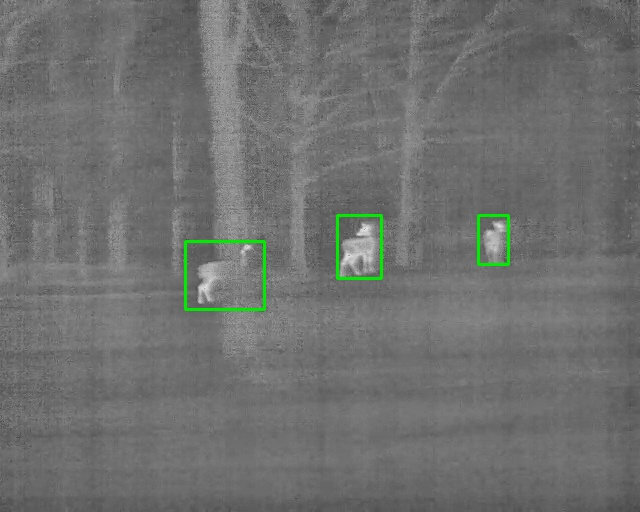
\includegraphics[width=0.228\textwidth]{figures/dataset/p3_gt.jpg} &
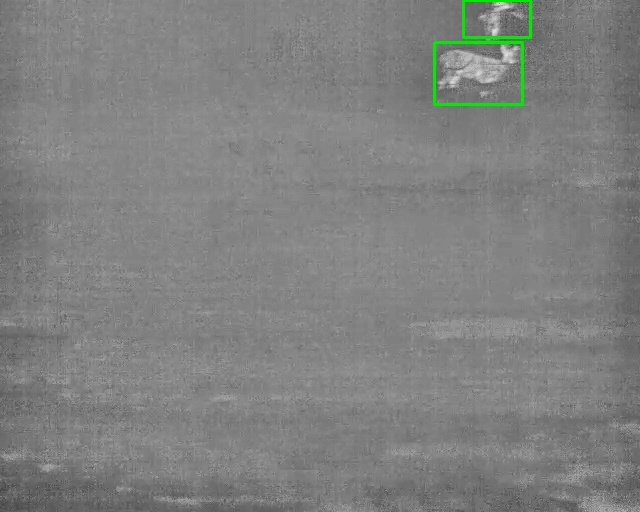
\includegraphics[width=0.228\textwidth]{figures/dataset/p4_gt.jpg} \\[2pt]
\small (\textbf{a}) two ranges & \small (\textbf{b}) close approach &
\small (\textbf{c}) group, three ranges & \small (\textbf{d}) mid-range pair \\
\end{tabular}
\caption{\textbf{Dataset examples.} Top row: raw thermal frames after the CLAHE
normalization the detector is trained and evaluated with. Bottom row: the same frames with
their ground-truth boxes. Panels show the \emph{large} end of the corpus for legibility at
print scale.\label{fig:dataset}}
\end{figure}

\begin{table}[H]
\caption{\textbf{Dataset composition.} 32 thermal road-transect videos from four Illinois
sites, $640\times512$ at 60\,fps, a single annotated class. Splits are by video and
site-stratified. Rows count the frames \emph{extracted} for detector training, not the
521,930 frames of the corpus; the complete track annotation is 21,646 boxes, of which the
12,903 here fall inside the extracted frames.\label{tab:dataset}}
\centering
\begin{tabularx}{\textwidth}{lRRRRR}
\toprule
\textbf{Split} & \textbf{Videos} & \textbf{Frames} & \textbf{With Deer} & \textbf{Empty} & \textbf{Boxes} \\
\midrule
Train & 19 & 12,852 & 5013 & 7839 & 7547 \\
Val   &  4 &  2337 &   935 & 1402 & 2564 \\
Test  &  9 &  3725 & 1490 & 2235 & 2792 \\
\midrule
\textbf{Total} & \textbf{32} & \textbf{18,914} & \textbf{7438} & \textbf{11,476} & \textbf{12,903} \\
\bottomrule
\end{tabularx}
\end{table}

Two frame counts appear in this paper and they measure different things. The 32 videos
contain 521,930 frames in total, and \emph{every} deer in \emph{every} frame of all 32 is
annotated in the Computer Vision Annotation Tool (CVAT) as a member of an individual track: that annotation is the 236 tracks and
21,646 boxes quoted above, and it is what ``fully annotated'' refers to. Training a detector
on all 521,930 frames would be wasteful rather than helpful, because at 60\,fps consecutive frames are near-duplicates, so the detector dataset of \cref{tab:dataset} is an extraction from
that annotation: 18,914 frames sampled around annotated activity together with explicit
negatives, carrying the 12,903 boxes that fall inside them. The 21,646 figure is therefore the
size of the ground truth, the 12,903 the size of the detector's training signal, and the
counting evaluation of \cref{sec:counting} always runs against the former, on whole videos
decoded end to end, never against the sampled subset.

Of the 18,914 extracted frames, 7438 contain at least one deer and 11,476 are explicit
negatives; background frames matter, since a survey system must not fire on warm rocks or
structures. The 236 animals are unevenly distributed across the four sites: SHB contributes 132 (56\% of
the corpus), TON 51, SHW 38 and MAS 15. One TON track is marked outside on every frame, the
animal being occluded throughout, so it can never be detected; \textbf{235 animals are
detectable and every detection and counting denominator in this paper is 235}, while 236
remains the count of annotated individuals. That imbalance is not incidental: SHB is the dense-group site where most of our counting error concentrates
(\cref{sec:counting}), and MAS is small enough that its per-site figures should be read as
indicative only.

Every individual deer is annotated in CVAT as a distinct \emph{track}. This is the property
the paper depends on: one track is one animal, so the same annotation simultaneously serves
as per-frame detection ground truth, as association ground truth, as count ground truth
(the number of tracks in a video), and, as \cref{sec:analysis} exploits, as identity labels for the appearance analysis of \cref{sec:reid}.

We split by \emph{video}, never by frame, and stratify by site so all four sites appear in
each split, the deployment target is these same sites, and a frame-level split would leak
near-duplicate frames across the boundary. The result is 19 training videos (12,852 images),
4 validation (2337) and 9 test (3725), allocated by animal count to roughly 65/19/16\%.

Throughout the paper, \textbf{``held out'' means the 13 validation and test videos the
detector never trained on}, containing 83 of the 236 deer. \Cref{sec:counting} shows why
this distinction is not pedantic: counting accuracy measured over all 32 videos, 19 of which
trained the detector, is 15.5 points higher than on held-out video alone.

\subsection{Object Scale}
\label{sec:scale}

The animals are small and the distribution is one-sided: median box $29\times24$ pixels
($\sqrt{\text{area}}=26.8$), 71\% below the COCO~\cite{lin2014coco} small-object threshold
of $32^2$, and \emph{zero} boxes in the COCO-large category. Resolution is therefore the
strongest single accuracy lever, which motivates the ablation in \cref{sec:detection}. The
one-sidedness has a second consequence, developed in \cref{sec:analysis}: no box in the
training split exceeds 96 pixels, and detector performance falls on the few animals that appear larger: the upper tail of the scale distribution is as under-served as the lower
one, and is far less often checked.

\subsection{Counting Pipeline}
\label{sec:pipeline}

\begin{figure}[htbp]
\begin{adjustwidth}{-\extralength}{0cm}
  \centering
  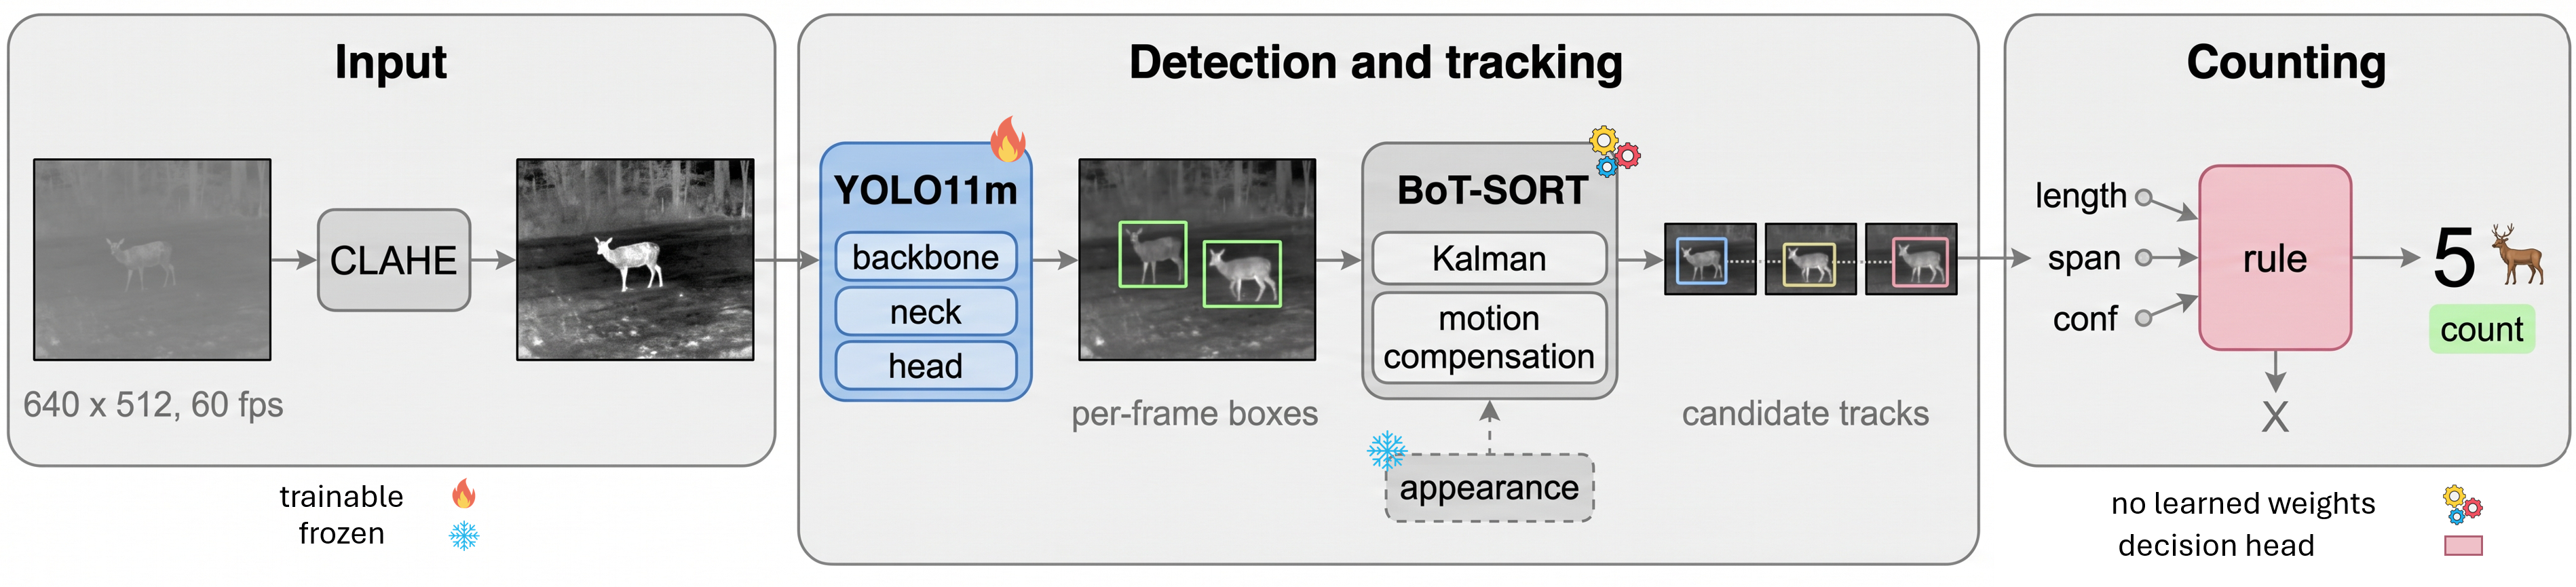
\includegraphics[width=\fulllength]{figures/wildlife_pipeline.png}
\end{adjustwidth}
  \caption{\textbf{The TRACT counting pipeline.} Thermal frames are contrast-normalized,
detected per frame, associated into candidate tracks, and filtered by a three-parameter
  confirmation rule; the count is the number of accepted tracks. Dashed components were
  ablated and are not used. Frames are illustrative.\label{fig:pipeline}}
\end{figure}

\Cref{fig:pipeline} shows the system, which we refer to as \textbf{TRACT} (Thermal
Road-transect Animal Counting and Tracking). The name denotes a composition rather than an
architecture: every component is standard, and the assembly (contrast normalisation, detection, motion-compensated tracking, orphan recovery and a calibrated confirmation rule) is what is arranged for counting rather than for detection. Detections from YOLO11m at
640\,px are associated by
BoT-SORT~\cite{aharon2022botsort} with sparse-optical-flow global motion compensation (mandatory here, since the whole frame translates as the vehicle moves), producing candidate tracks. One point of terminology belongs here, because the association stage is easily
mistaken for something it is not. \textbf{The reported system runs with BoT-SORT's appearance term disabled and does not attempt to recognise individual animals.} It associates detections into tracks within
a single video using motion and geometry, which prevents an animal from being counted twice in
one transect; it makes no claim to recognise an individual animal, and could not, since
\cref{sec:reid} shows that at a median $29\times24$ pixels a two-number size descriptor
out-performs a pretrained appearance backbone. We call this \emph{track association} throughout. Where appearance appears in this paper it is an
\emph{ablation} (pool G of \cref{sec:inversion}) or a probe of how much identity signal the
imagery carries (\cref{tab:reid}), never a component of the counting results we report.

Only one component of the system is gradient-trained. The tracker's Kalman filter,
motion compensation and association carry no weights at all, and the confirmation rule's three
parameters are fitted by grid search rather than by training. The detector is also not the one
with the best AP$_{50}$, and the choice is deliberate:
\cref{sec:choosing} selects on the precision-weighted $F_{0.5}$ instead, because the
confirmation stage that consumes these detections must reject tens of thousands of false
candidates against roughly two hundred true ones and therefore pays far more for a false
positive than for a false negative. That section also verifies the choice end to end, running
the highest-AP$_{50}$ model through this same pipeline and finding that it counts fewer
animals. A confirmation stage then decides which candidates are real, distinct animals. The
count is the number of accepted candidates.

The confirmation baseline is a three-parameter rule: accept a candidate if it persists for
at least $m$ frames, spans at least $s$ seconds, and the mean of its five highest per-frame
detector confidences is at least $c$. Under the held-out protocol (\cref{sec:heldout}) the
swept values are $m\ge20$, $s\ge0$, $c\ge0.65$. Note that $c$ is a property of the
\emph{track}, not of any single frame: a low-confidence frame is never discarded, it
continues to extend the track, and a candidate is rejected only when its five \emph{best}
frames average below $c$. \Cref{sec:sensitivity} measures what each of the three
parameters is worth.

We additionally recover \emph{orphan} detections, those the tracker returns without a
track identity, by linking detections within a temporal gap and a scale-normalized
distance into pseudo-tracks. Without this, single-frame animals are discarded entirely; with
it, 17 animals are recovered.

\subsection{Calibrated Per-Animal Confidence}
\label{sec:calibration}

A survey system that cannot say how sure it is cannot be audited. We calibrate a per-track
posterior for ``this track is on a real animal'' and report it with every counted animal:
\textbf{92.1\% of counted animals carry confidence $\ge0.80$} (mean 0.965, area under the ROC curve 0.893), and
793 low-confidence tracks are flagged for human review rather than auto-counted. We also
propagate per-track probabilities into a Poisson-binomial standard deviation on each video's
count, giving an uncertainty interval rather than a point estimate.

The calibrator is \textbf{isotonic regression fitted on the validation videos only}, mapping
the confirmer's raw score to a probability; no held-out video contributes to the fit. Isotonic
rather than Platt scaling because the raw score is not sigmoidal in the log-odds and a
monotone step function makes no shape assumption; the cost is that the output takes a finite
number of levels, 46 of them on held-out video.

\Cref{tab:calib} reports whether the resulting number behaves like a probability on videos the
calibrator never saw, scoring a track as positive when it is the \emph{primary} track of a real animal; duplicates count as negatives, which is the decision the counting stage
actually makes. Over all 2211 held-out candidate tracks the expected calibration error (ECE) is 0.004 and the Brier score 0.017 against 0.029 for a constant predictor at the base rate. That
aggregate is generous, because 74\% of candidates sit at the isotonic floor where no decision
is ever taken; restricted to the 316 tracks in the decision region the expected calibration
error is 0.034 and the Brier score 0.093 against 0.148. Both are honest and the second is the
one a practitioner should read. One caveat belongs with them: isotonic saturates, so the top
level reports 1.000 on 13 held-out tracks whose true positive rate is 0.846. Confidence at the
very top of the scale is optimistic by roughly 15 points, and the flag-for-review band, not
the top of the scale, is where the calibrated number earns its keep.

\begin{table}[H]
\caption{\textbf{Reliability of the per-track posterior} on the 13 held-out videos, against
the isotonic calibrator fitted on validation videos only. Positives are primary tracks;
duplicates are negatives. The constant-predictor column is the Brier score of always
predicting the base rate, so the gap is the skill the posterior
adds.\label{tab:calib}}
\centering\footnotesize
\begin{tabularx}{\textwidth}{LCCCCC}
\toprule
\textbf{Scope} & \textbf{Tracks} & \textbf{Base rate} & \textbf{ECE} & \textbf{Brier} & \textbf{Constant} \\
\midrule
All held-out candidates & 2211 & 0.030 & 0.004 & 0.017 & 0.029 \\
Decision region ($p>0.01$) & 316 & 0.180 & 0.034 & 0.093 & 0.148 \\
\midrule
Fit videos, for reference & 4797 & 0.029 & 0.003 & 0.017 & 0.029 \\
\bottomrule
\end{tabularx}
\end{table}

Raw detector confidence cannot serve this purpose: no track in the corpus exceeds 0.90 and
the median counted track sits at 0.74, because the animals are 27 pixels. The requirement is
only meaningful against a calibrated posterior. \Cref{fig:evidence} shows why a score must be
per track rather than per frame: the raw confidence varies by 0.15 across frames of the same
animal (Animal B, 0.66--0.81) even where every frame is a clean detection, so no single
frame's value characterises the track. It also shows the audit trail: every counted animal is exported as a contact sheet of its own track, one panel per sampled frame with elapsed time
and per-frame score beneath, so a human can verify any individual count against the frames
that produced it.

\begin{figure}[htbp]
  \centering
  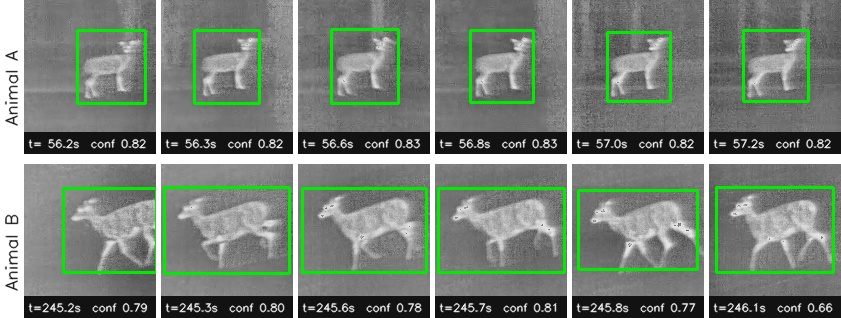
\includegraphics[width=0.86\linewidth]{figures/evidence_two.jpg}
  \caption{\textbf{Per-animal evidence, two individuals.} Each row is one animal's own
  track, one panel per sampled frame, with elapsed time and raw per-frame detector confidence
  beneath. Both animals are from videos the detector never trained on.\label{fig:evidence}}
\end{figure}

\subsection{Matching Criterion}
\label{sec:criterion}

A detection metric asks whether a predicted box \emph{localizes} an animal; a survey asks
whether the animal was \emph{noticed}. On a 27-pixel target these diverge sharply: a box
offset by six pixels falls below IoU 0.5 and is scored as both a false positive and a false
negative, while for counting it has correctly found the animal. We therefore evaluate under four matching rules: intersection over union (IoU) $\geq$0.50, IoU$\geq$0.30, centre-in-box and \emph{any overlap}, and treat the last as the counting criterion, reporting it as presence or counting recall
and never as mAP, with the strict criterion alongside it everywhere.

The criterion is validated against centre-in-box, an independent counting-oriented rule that
accepts a prediction only when its centre falls inside the animal and so rejects oversized
boxes outright. The two agree to within 0.032 F1 across all eleven models, so the
conclusions rest on two criteria agreeing rather than on one being chosen. Precision is
reported alongside recall throughout, which additionally constrains box quality.

\subsection{Decomposing Counting Error}
\label{sec:decomposition}

This is the paper's main instrument. Let $G$ be the ground-truth animals in a video and $C$
the candidate tracks a pipeline produces. For each $g\in G$ we define:

\begin{itemize}[leftmargin=*,labelsep=4.5mm]
\item \reachedq: $g$ is touched, on at least one frame, by at least one candidate. If
an animal is not \reachedq, no downstream stage can recover it; this measures
\textbf{detection and tracking}.
\item \primaryq: among the candidates touching $g$, the one that covers $g$ on the most
frames is not simultaneously the best cover for some other animal. Two animals sharing a
single best-covering candidate are indistinguishable to any decision rule that emits one
count per track; this measures \textbf{association}.
\item \countedq: the confirmation stage accepted a candidate covering $g$. This measures
\textbf{confirmation}, and it is the end-to-end result.
\end{itemize}

The three are nested, $\countedq \le \primaryq \le \reachedq \le |G|$, and the gaps
attribute error to the three stages. We report all three for every configuration; reporting
only the last, as is conventional, makes a detection miss and a confirmation miss look identical.

We report mean absolute error in animals per video (MAE), signed bias, and a \emph{counted}
fraction. The latter is $\sum_v \min(\hat{c}_v, c_v) / \sum_v c_v$, capped per video so that
over-counting in one video cannot mask misses in another.

We also report a stricter identity-matched variant, the fraction of individual animals
covered by an \emph{accepted} candidate, which \cref{sec:counting} shows is 10 points
lower; the capped aggregate credits a video for predicting the right \emph{number} even
when the accepted tracks do not land on the animals.

Counting quantities carry 95\% intervals throughout. Proportions over the 83 held-out animals
use the Wilson score interval, and means over the 13 held-out videos use a $t$-interval on the
per-video values. These are sampling intervals over the corpus, and with 83 animals they are
wide: a three-animal difference is not resolvable. We deliberately do \emph{not} attach
intervals to the detection metrics of \cref{sec:detection}. Each architecture was trained
once, so a bootstrap over the test images would produce a narrow interval that describes
test-set sampling while saying nothing about the training variance that actually separates one
architecture from another, a precision the experiment does not support.

\subsection{Held-Out Protocol}
\label{sec:heldout}

Counting runs process all 32 videos, but the detector trained on 19 of them, and the
hand-tuned confirmation rule is conventionally swept on the same videos it is reported on.
Both leaks inflate the result. Our protocol closes both: \textbf{sweep the rule on the 19
detector-training videos, freeze it, and report on the 13 held-out videos}. Learned
confirmers are trained and thresholded under the identical split, so the comparison in
\cref{sec:learned} is like-for-like.

\begin{table}[H]
\caption{\textbf{Why the held-out protocol matters.} Evaluating on all 32 videos, as an in-sample pipeline evaluation would, reports 81.8\% coverage. On video the detector never trained on
it is 66.3\%. Both figures use the capped per-video fraction of \cref{sec:decomposition}; the
uncapped ratio of predicted to true animals reads 89.0\% and 69.9\% respectively, and is the
more flattering of the two because over-counting one video offsets misses in another.\label{tab:leak}}
\centering
\begin{tabularx}{\textwidth}{lRRR}
\toprule
\textbf{Evaluation Scope} & \textbf{Videos} & \textbf{Deer} & \textbf{Coverage} \\
\midrule
Detector-training videos & 19 & 153 & 90.2\% \\
\textbf{Held out (val + test)} & \textbf{13} & \textbf{83} & \textbf{66.3\%} \\
All 32 (the default) & 32 & 236 & 81.8\% \\
\bottomrule
\end{tabularx}
\end{table}

The protocol is worth 15.5 points (\cref{tab:leak}): counting accuracy measured over all 32
videos is 81.8\%, and on the 13 held-out videos it is 66.3\%. One qualification belongs
here, because the paper's argument is about evaluation rigour. Four of the 13 held-out
videos are the detector's \emph{validation} split. No gradient was computed on them, but
they were used for checkpoint selection, so they are held out in the sense that matters for
the confirmation rule and only partly held out for the detector. They carry 45 of the 83
animals. We state this rather than reporting on the 9 test videos alone because the
confirmation rule, the subject of the paper, saw none of the 13, and because splitting
the held-out set further would leave 38 animals to carry every counting conclusion.
